\documentclass[11pt,a4paper]{article}
\usepackage[spanish,es-nodecimaldot]{babel}	% Utilizar español
\usepackage[utf8]{inputenc}					% Caracteres UTF-8
\usepackage{graphicx}						% Imagenes
\PassOptionsToPackage{hyphens}{url}\usepackage[hidelinks]{hyperref}			% Poner enlaces sin marcarlos en rojo
\usepackage{fancyhdr}						% Modificar encabezados y pies de pagina
\usepackage{float}							% Insertar figuras
\usepackage[textwidth=390pt]{geometry}		% Anchura de la pagina
\usepackage[nottoc]{tocbibind}				% Referencias (no incluir num pagina indice en Indice)
\usepackage{enumitem}						% Permitir enumerate con distintos simbolos
\usepackage[T1]{fontenc}					% Usar textsc en sections
\usepackage{amsmath}						% Símbolos matemáticos

% Comando para poner el nombre de la asignatura
\newcommand{\asignatura}{Arquitectura y Computación de Altas Prestaciones}
\newcommand{\autor}{Vladislav Nikolov Vasilev}
\newcommand{\titulo}{Trabajo 1}
\newcommand{\subtitulo}{AMD: Arquitectura modular para procesadores}
\newcommand{\rama}{Ingeniería de Computadores}

% Configuracion de encabezados y pies de pagina
\pagestyle{fancy}
\lhead{\autor{}}
\rhead{\asignatura{}}
\lfoot{Grado en Ingeniería Informática}
\cfoot{}
\rfoot{\thepage}
\renewcommand{\headrulewidth}{0.4pt}		% Linea cabeza de pagina
\renewcommand{\footrulewidth}{0.4pt}		% Linea pie de pagina

\begin{document}
\pagenumbering{gobble}

% Pagina de titulo
\begin{titlepage}

\begin{minipage}{\textwidth}

\centering

%
\includegraphics[scale=0.5]{img/ugr.png}\\

\includegraphics[scale=0.3]{img/logo_ugr.jpg}\\[1cm]

\textsc{\Large \asignatura{}\\[0.2cm]}
\textsc{GRADO EN INGENIERÍA INFORMÁTICA}\\[1cm]

\noindent\rule[-1ex]{\textwidth}{1pt}\\[1.5ex]
\textsc{{\Huge \titulo\\[0.5ex]}}
\textsc{{\Large \subtitulo\\}}
\noindent\rule[-1ex]{\textwidth}{2pt}\\[3.5ex]

\end{minipage}

%\vspace{0.5cm}
\vspace{0.7cm}

\begin{minipage}{\textwidth}

\centering

\textbf{Autor}\\ {\autor{}}\\[2.5ex]
\textbf{Rama}\\ {\rama}\\[2.5ex]
\vspace{0.3cm}


\includegraphics[scale=0.3]{img/etsiit.jpeg}

\vspace{0.7cm}
\textsc{Escuela Técnica Superior de Ingenierías Informática y de Telecomunicación}\\
\vspace{1cm}
\textsc{Curso 2019-2020}
\end{minipage}
\end{titlepage}

\pagenumbering{arabic}

\newpage

\setlength{\parskip}{1em}

\section*{Mercado actual}

Durante la última década, Intel ha tenido una cuota de mercado muy superior a la de sus
competidores, dejándolos en segundo plano. Y esto es lo que le ha venido pasando a AMD durante
este tiempo, ya que sus procesadores habían caído en el olvido frente a los de las familias Core y
Xeon. Los procesadores de AMD no eran capaces de competir contra los de Intel por mucho que se
mejorasen, y lentamente, la compañía fue perdiendo cuota de mercado frente al titán del sector.

No obstante, con el lanzamiento de los procesadores con arquitectura Zen en 2017 y el posterior
lanzamiento de los procesadores con la arquitectura Zen 2 durante 2019, Intel ha comenzado a
perder cuota de mercado y AMD a ganarla, llegando ambos a niveles que no se habían visto en
ninguno de ellos desde el tercer cuatrimestre de 2006.

\begin{figure}[H]
  \centering
  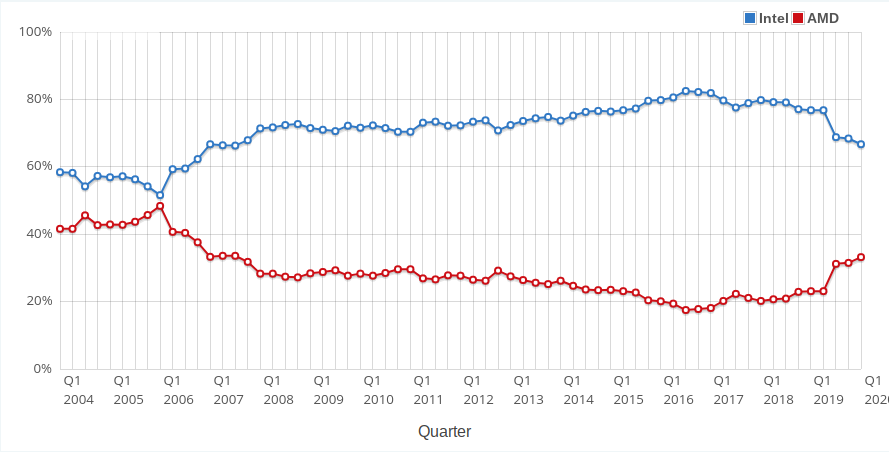
\includegraphics[scale=0.6]{img/cuota-mercado-intel-amd}
  \caption{Cuota de mercado de los procesadores en uso de Intel y AMD desde 2004 hasta la
  actualidad \cite{passmark}.}
\end{figure}

Aunque en el gráfico se puede ver que Intel sigue dominando el mercado, la tendencia es a la baja,
mientras que el de AMD es a la alza. El aumento de cuota de AMD se debe a que ha sabido ofrecer
procesadores con un rendimiento superior a los de Intel a un precio mucho más asequible, tanto
para la gama de servidores como en la media.

Y es que, en la actualidad, la única forma que tiene Intel de competir es reduciendo los precios
de sus procesadores, tanto en la gama media como en la de servidores. A pesar de eso, los
procesadores de AMD son, en la actualidad, bastante superiores a los de Intel, e incluso si tienen
el mismo precio, los de AMD son preferidos debido a su rendimiento superior y menor consumo. Por
tanto, la tendencia actual del mercado parece que va a continuar durante algún tiempo más, hasta
que o bien AMD empiece a dominar el mercado o Intel dé un golpe sobre la mesa ofreciendo una
mejora revolucionaria. Pero, por el momento, parece que AMD va a continuar ganando cuota de
mercado con sus procesadores.

De hecho, los precios de los procesadores de alto rendimiento de Intel han tenido que rebajar su
precio de manera descomunal para poder competir con AMD, algo nunca visto por parte de la
compañía. Algunos ejemplos son el Intel Core i9-10980X, que ha visto rebajado su precio un 50,40
\% (de 1975 \$ a 979\$); el Intel Core i9-10940X ahora es un 43,40\% más barato (1387\$ a 784\$);
el Intel Core i9-10920X pasa de los 1189 a los 689 dólares (-42\%); y el Intel Core i9-10900X pasa
de costar 989 a 590 dólares (40,30\%).

\begin{figure}[H]
  \centering
  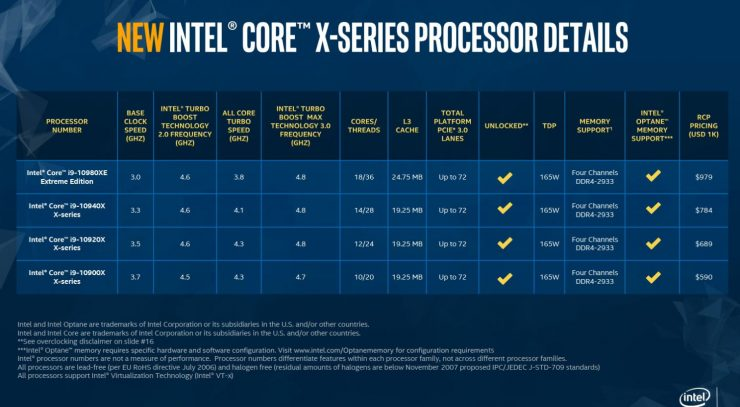
\includegraphics[scale=0.5]{img/procesadores-intel}
  \caption{Serie de procesadores Intel Core X \cite{chapuzas4}.}
\end{figure}

Además de todo esto, AMD está empezando a ganar terreno en el mercado de los superordenadores.
Recientemente, AMD ha obtenido un contrato para la construcción del que promete ser el
superordenador más rápido del mundo, \textbf{El Capitan}, utilizando tanto procesadores Epyc como
gráficas Radeon. También han acordado la construcción de otro superordenador para la National
Oceanic and Atmospheric Administration de EE.UU. Y no solo eso, ya que también están construyendo
otro superordenador, \textbf{Frontier}, para el Oak Ridge National Laboratory,  el cual se espera
que esté listo en 2021. Por una parte, esto es una gran victoria para AMD, ya que está empezando a
ganar cuota en un mercado que antaño era dominado exclusivamente por Intel. Por otra parte,
significa que la gente confía más en el rendimiento que ofrecen sus procesadores que en los de su
competidor directo, y les asegura que van a tener más demanda en los próximos años.

\begin{figure}[H]
  \centering
  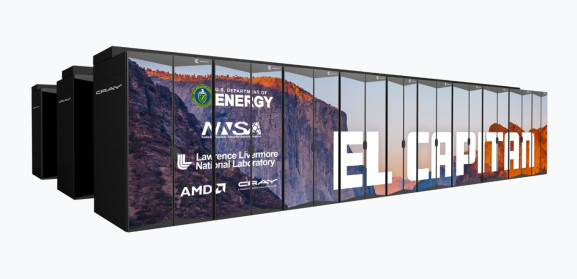
\includegraphics[scale=0.7]{img/amd-el-capitan}
  \caption{Superordenador \textbf{El Capitan} \cite{venturebeat}.}
\end{figure}

\newpage

\begin{thebibliography}{20}

\bibitem{passmark}
PassMark Software. \textit{AMD vs Intel Market Share}
\\\url{https://www.cpubenchmark.net/market_share.html}

\bibitem{chapuzas4}
El Chapuzas Informático. \textit{Intel anuncia oficialmente sus Cascade Lake-X y formaliza la rebaja de precio en hasta un 50\%}
\\\url{https://elchapuzasinformatico.com/2019/10/intel-cascade-lake-x-formaliza-la-rebaja-de-precio-en-hasta-un-50/}

\bibitem{venturebeat}
VentureBeat. \textit{AMD’s top supercomputer wins are a big moment in ‘heated competition’}
\\\url{https://venturebeat.com/2020/03/05/amds-top-supercomputer-wins-are-a-big-moment-in-heated-competition/}

\bibitem{xataka}
Xataka. \textit{AMD y Cray preparan un supercomputador bestial: 'Frontier' llegará a los 1,5 exaFLOPS de potencia en 2021}
\\\url{https://www.xataka.com/investigacion/amd-cray-preparan-supercomputador-bestial-frontier-llegara-a-1-5-exaflops-potencia-2021}

\bibitem{chapuzas1}
El Chapuzas Informático. \textit{Según PassMark, AMD ha alcanzado una cuota de mercado del 40\%, Intel retrocede 14 años}
\\\url{https://elchapuzasinformatico.com/2020/01/segun-passmark-amd-ha-alcanzado-una-cuota-de-mercado-del-40-intel-retrocede-14-anos/}

\bibitem{chapuzas1}
El Chapuzas Informático. \textit{Según PassMark, AMD ha alcanzado una cuota de mercado del 40\%, Intel retrocede 14 años}
\\\url{https://elchapuzasinformatico.com/2020/01/segun-passmark-amd-ha-alcanzado-una-cuota-de-mercado-del-40-intel-retrocede-14-anos/}

\bibitem{chapuzas2}
El Chapuzas Informático. \textit{Intel anuncia su 2ª Gen de CPUs Xeon Scalable, ahora un 60\% más baratos para competir con AMD}
\\\url{https://elchapuzasinformatico.com/2020/02/intel-anuncia-su-2a-gen-de-cpus-xeon-scalable-ahora-un-60-mas-baratos-para-competir-con-amd/}

\bibitem{chapuzas3}
El Chapuzas Informático. \textit{El Ryzen Threadripper 3990X llegará por 3.990\$ destrozando a 2x Intel Xeon Platinum 8280 de +20.000\$}
\\\url{https://elchapuzasinformatico.com/2020/02/el-ryzen-threadripper-3990x-llegara-por-3-990-destrozando-a-2x-intel-xeon-platinum-8280-de-20-000/}

\bibitem{chapuzas5}
El Chapuzas Informático. \textit{Intel reduciría el precio de sus procesadores de consumo para intentar frenar a los AMD Ryzen}
\\\url{https://elchapuzasinformatico.com/2020/01/intel-reduciria-el-precio-de-sus-procesadores-de-consumo-para-intentar-frenar-a-los-amd-ryzen/}

\bibitem{chapuzas6}
El Chapuzas Informático. \textit{Las CPUs AMD EPYC 7742 darán vida al superordenador encargado de predecir el tiempo en Europa}
\\\url{https://elchapuzasinformatico.com/2020/01/las-cpus-amd-epyc-7742-daran-vida-al-superordenador-encargado-de-predecir-el-tiempo-en-europa/}

\bibitem{chapuzas7}
El Chapuzas Informático. \textit{La NOAA adquiere un superordenador con 5120 procesadores AMD EPYC ROME}
\\\url{https://elchapuzasinformatico.com/2020/02/la-noaa-adquiere-un-superordenador-con-5120-procesadores-amd-epyc-rome/}

\bibitem{chapuzas8}
El Chapuzas Informático. \textit{AMD dará vida al superordenador de la Armada de los Estados Unidos con 290.304 núcleos Zen2 @ 7nm}
\\\url{https://elchapuzasinformatico.com/2020/02/amd-dara-vida-al-superordenador-de-la-armada-de-los-estados-unidos-con-290-304-nucleos-zen2-7nm/}

\bibitem{chapuzas9}
El Chapuzas Informático. \textit{AMD se lleva el contrato de «El Capitan», el superordenador más potente del mundo}
\\\url{https://elchapuzasinformatico.com/2020/03/amd-se-lleva-el-contrato-de-el-capitan-el-superordenador-mas-potente-del-mundo/}

\end{thebibliography}

\end{document}

